%% Include the picture as follows: \
% \begingroup
% \tikzset{every picture/.style={scale=1,radius=0.05,line width=0.4}}%
% \input{tikz/[filename].tex}%
% \endgroup
%
%% Want to add a label? Use node[<position>]{label},
%% where <position> is one of: below / above / left / right
% \fill (0,0) circle node[below]{$p_1$};
%% Want to give the point a different color?
% \fill[red] (0,0) circle;
%
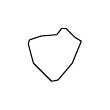
\begin{tikzpicture}
\draw (5.0789,3.9507) -- (4.9638,3.6711);
\draw (4.7664,4.0329) -- (4.5691,4.0164);
\draw (4.7007,3.4408) -- (4.4704,3.6711);
\draw (4.4046,3.9178) -- (4.4704,3.6711);
\draw (4.7829,3.4572) -- (4.7007,3.4408);
\draw (4.8816,4.1151) -- (4.9967,4.0000);
\draw (4.4211,3.9671) -- (4.5691,4.0164);
\draw (4.8322,4.1151) -- (4.8816,4.1151);
\draw (4.8322,4.1151) -- (4.7664,4.0329);
\draw (4.9967,4.0000) -- (5.0789,3.9507);
\draw (4.4211,3.9671) -- (4.4046,3.9178);
\draw (4.9638,3.6711) -- (4.7829,3.4572);
\fill (4.4211,3.9671) circle;
\fill (4.5691,4.0164) circle;
\fill (4.9967,4.0000) circle;
\fill (5.0789,3.9507) circle;
\fill (4.9638,3.6711) circle;
\fill (4.7829,3.4572) circle;
\fill (4.7007,3.4408) circle;
\fill (4.4704,3.6711) circle;
\fill (4.4046,3.9178) circle;
\fill (4.8322,4.1151) circle;
\fill (4.8816,4.1151) circle;
\fill (4.7664,4.0329) circle;
\end{tikzpicture}
